\section{The algorithmic agent}

%%%%%%%%%%%%%%%%%%%%%%%%%%%%%%%%%%%%%%%%%%%%%%%%%%
\begin{frame}[label=ladila]{The algorithmic agent}
Minimal set of elements needed for a homeostatic algorithmic system in an information bath. Can be connected with neurobiology.
 \begin{center}
  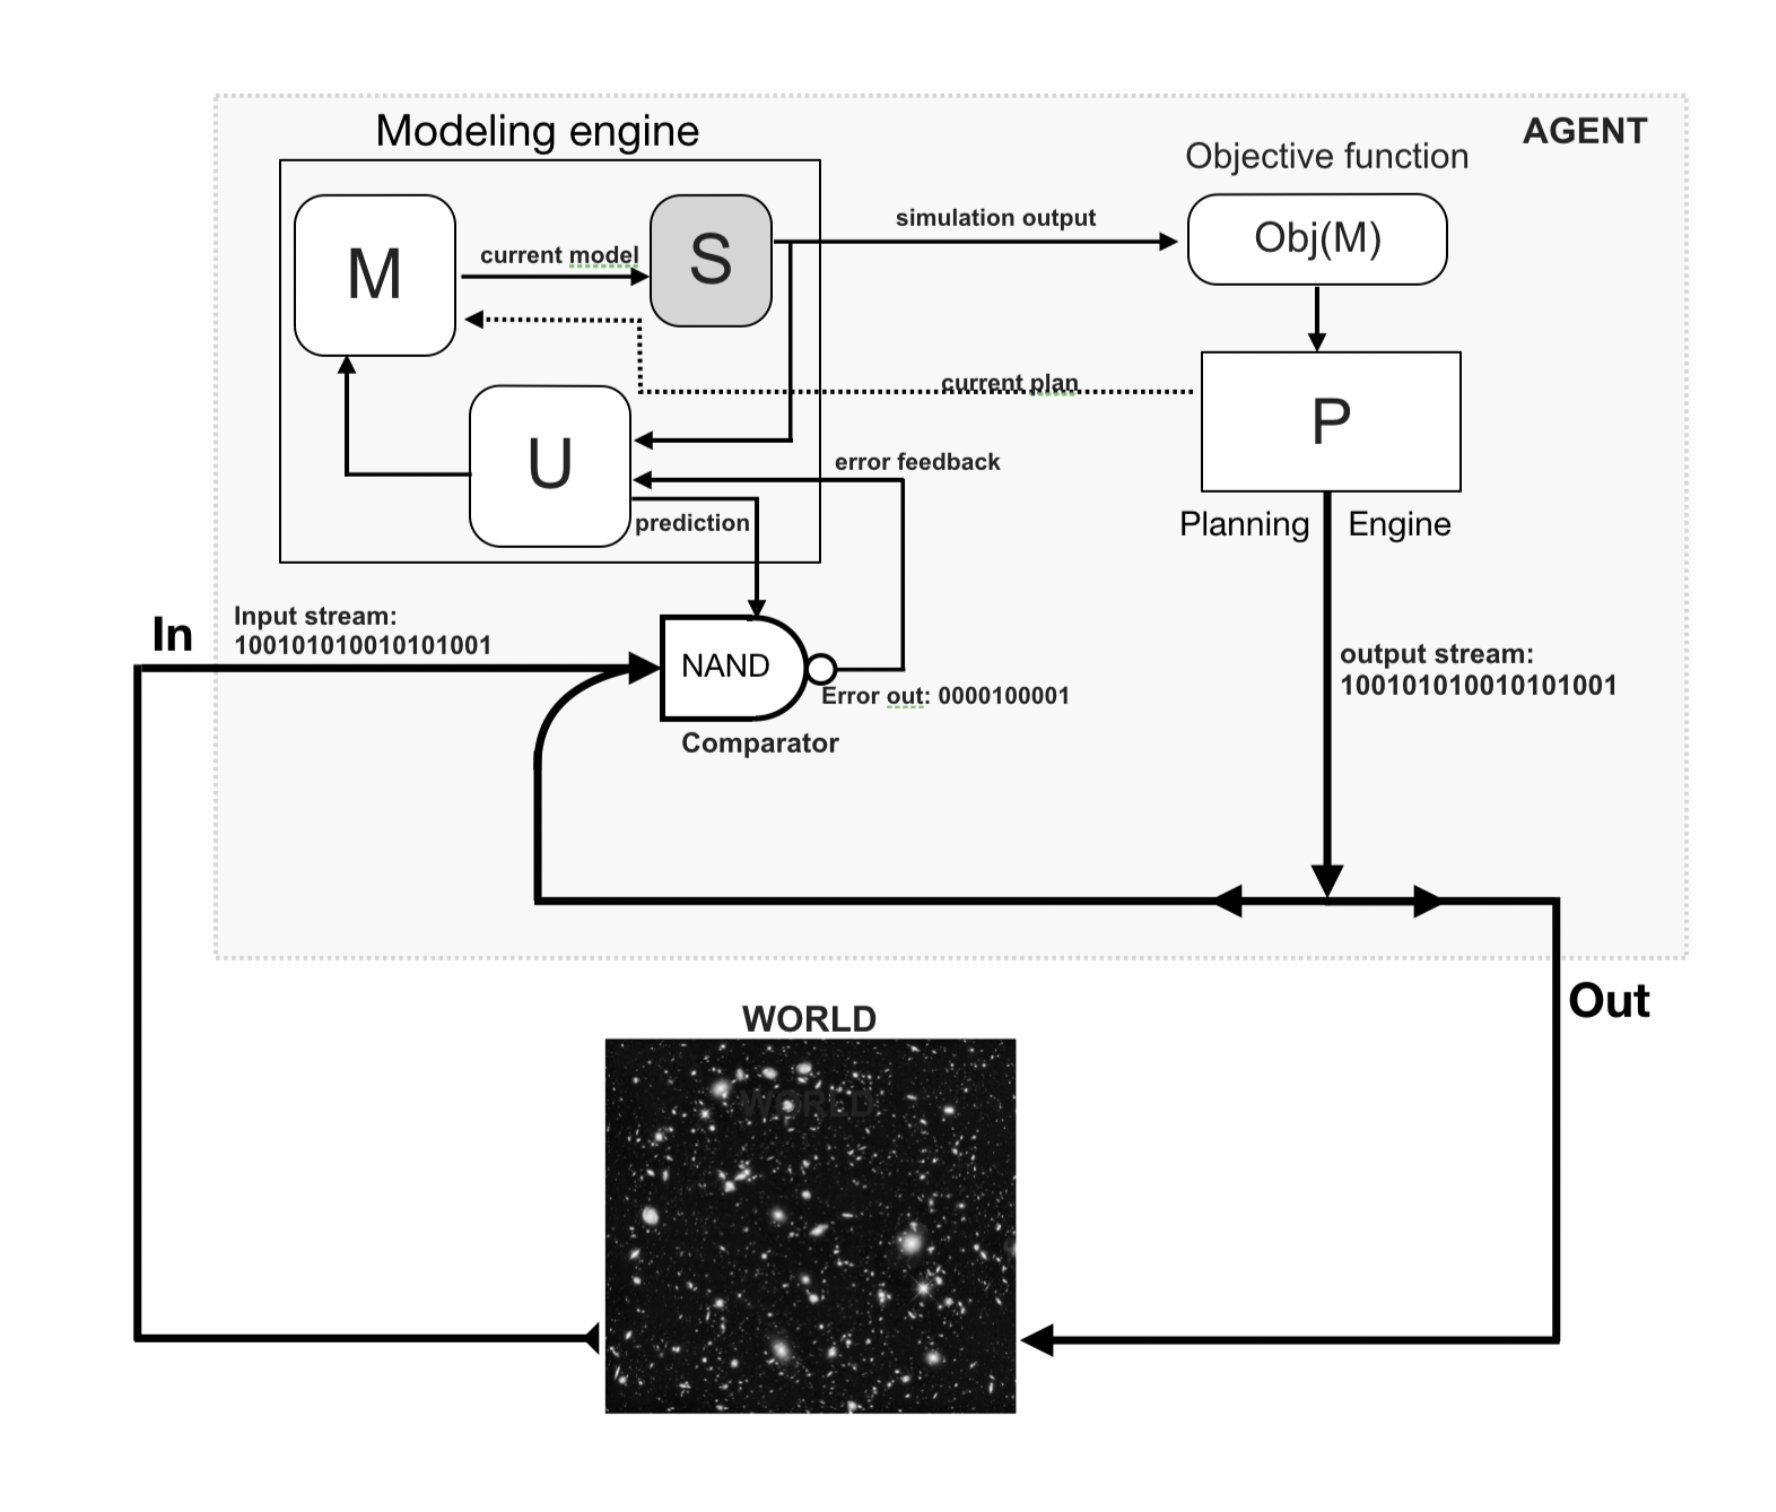
\includegraphics[height=6cm]{img/agent.png}
  \end{center}

\end{frame}



%%%%%%%%%%%%%%%%%%%%%%%%%%%%%%%%%%%%%%%%%%%%%%%%%%
\begin{frame}[label=ladila]{The algorithmic event of \SEP}
Theories of cortical processing emphasize the separation of forward and backward information flow in the cortex also mirrored at the level of single cortical pyramidal cells \citep{CarhartHarris2019,Aru2020}. {\bf Comparator} implemented hierarchically in L5 P cells.

 
  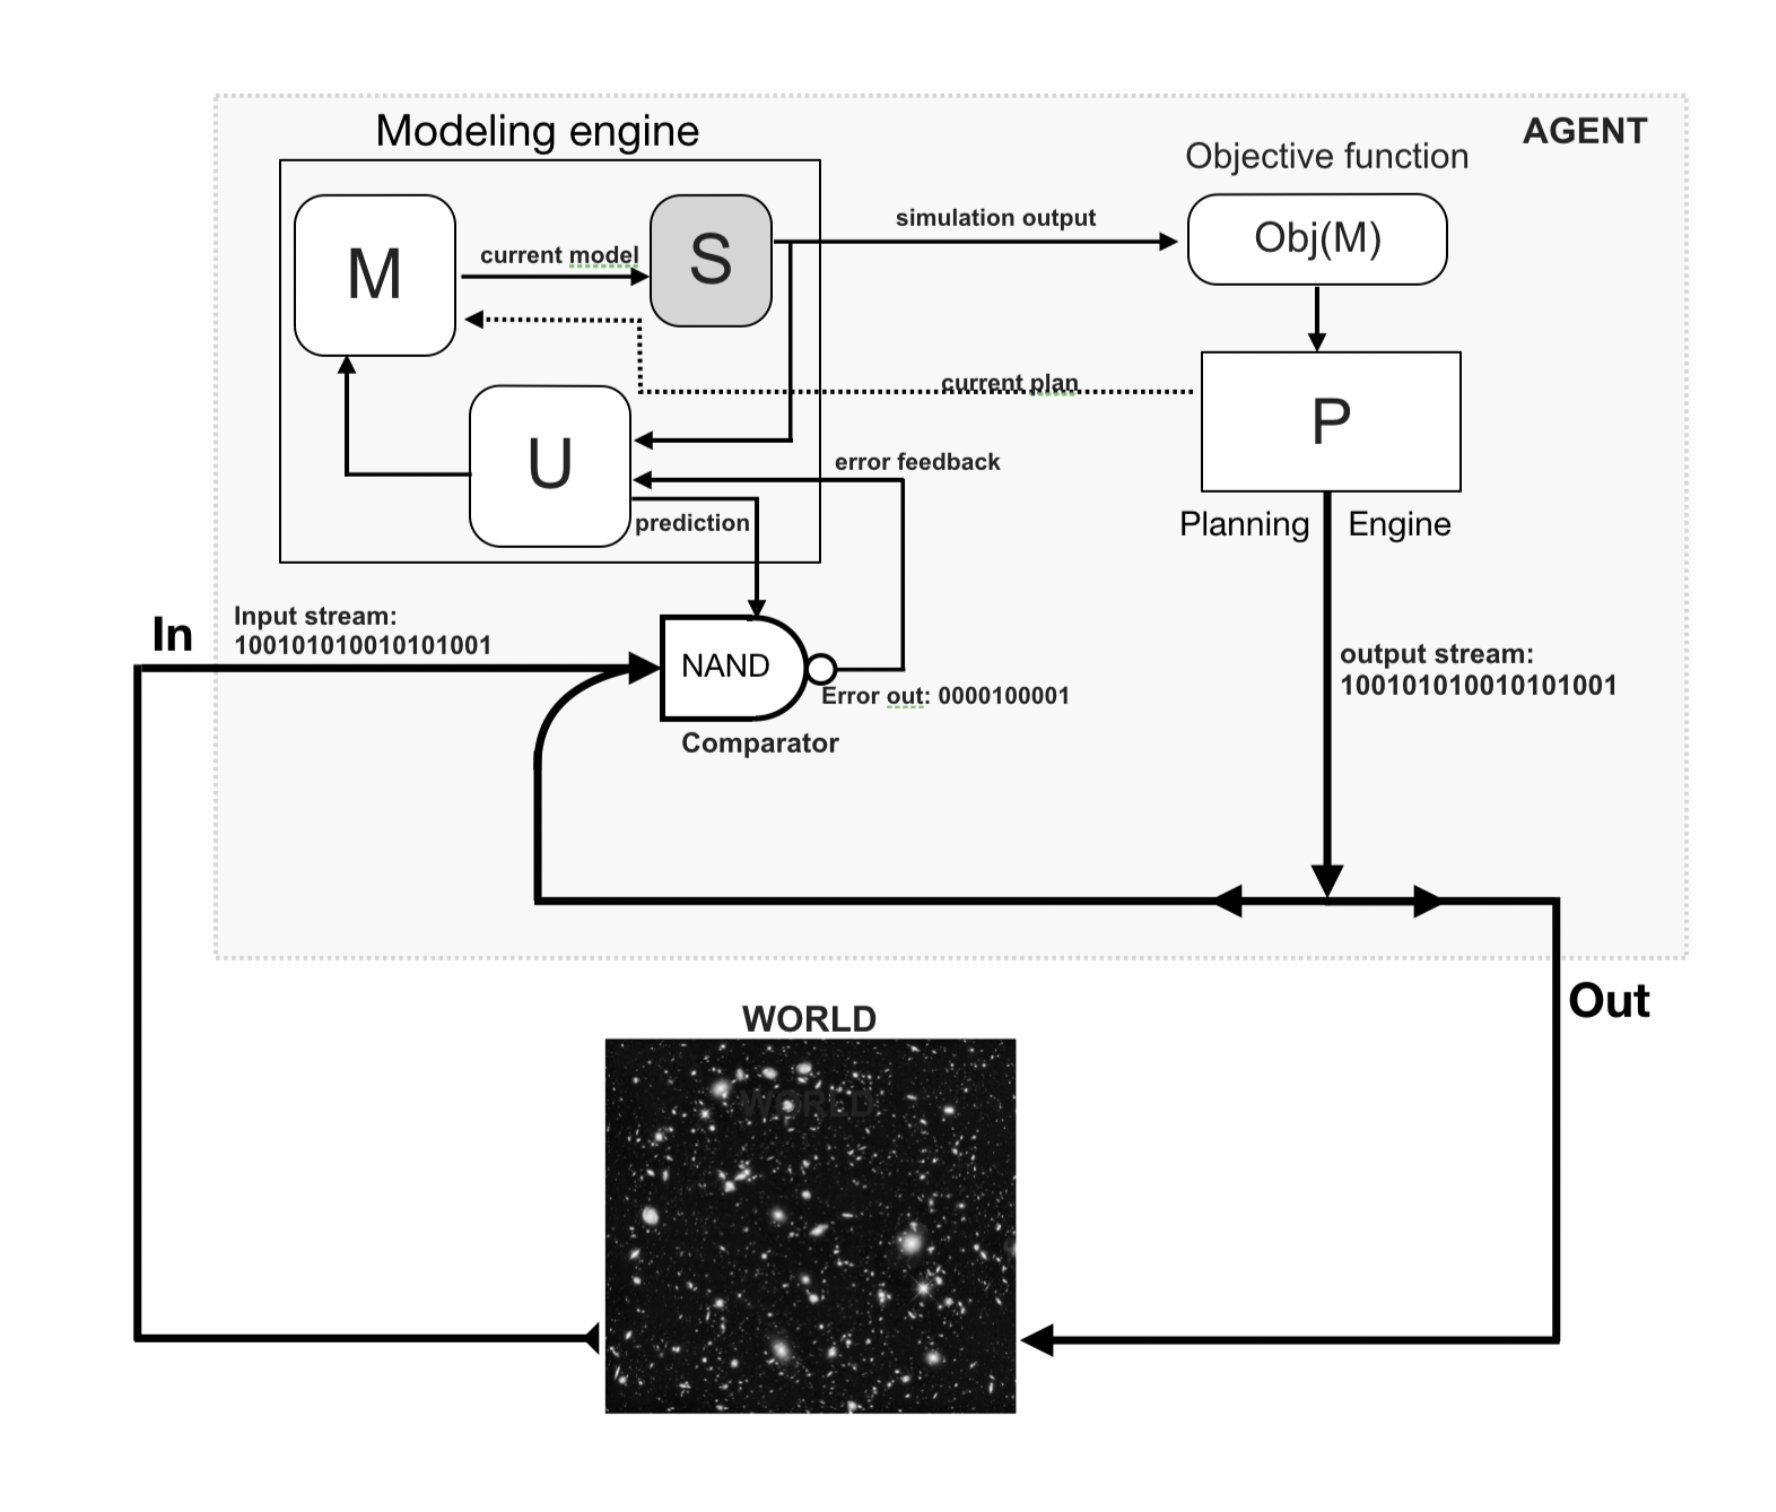
\includegraphics[height=4.cm]{img/agent.png}
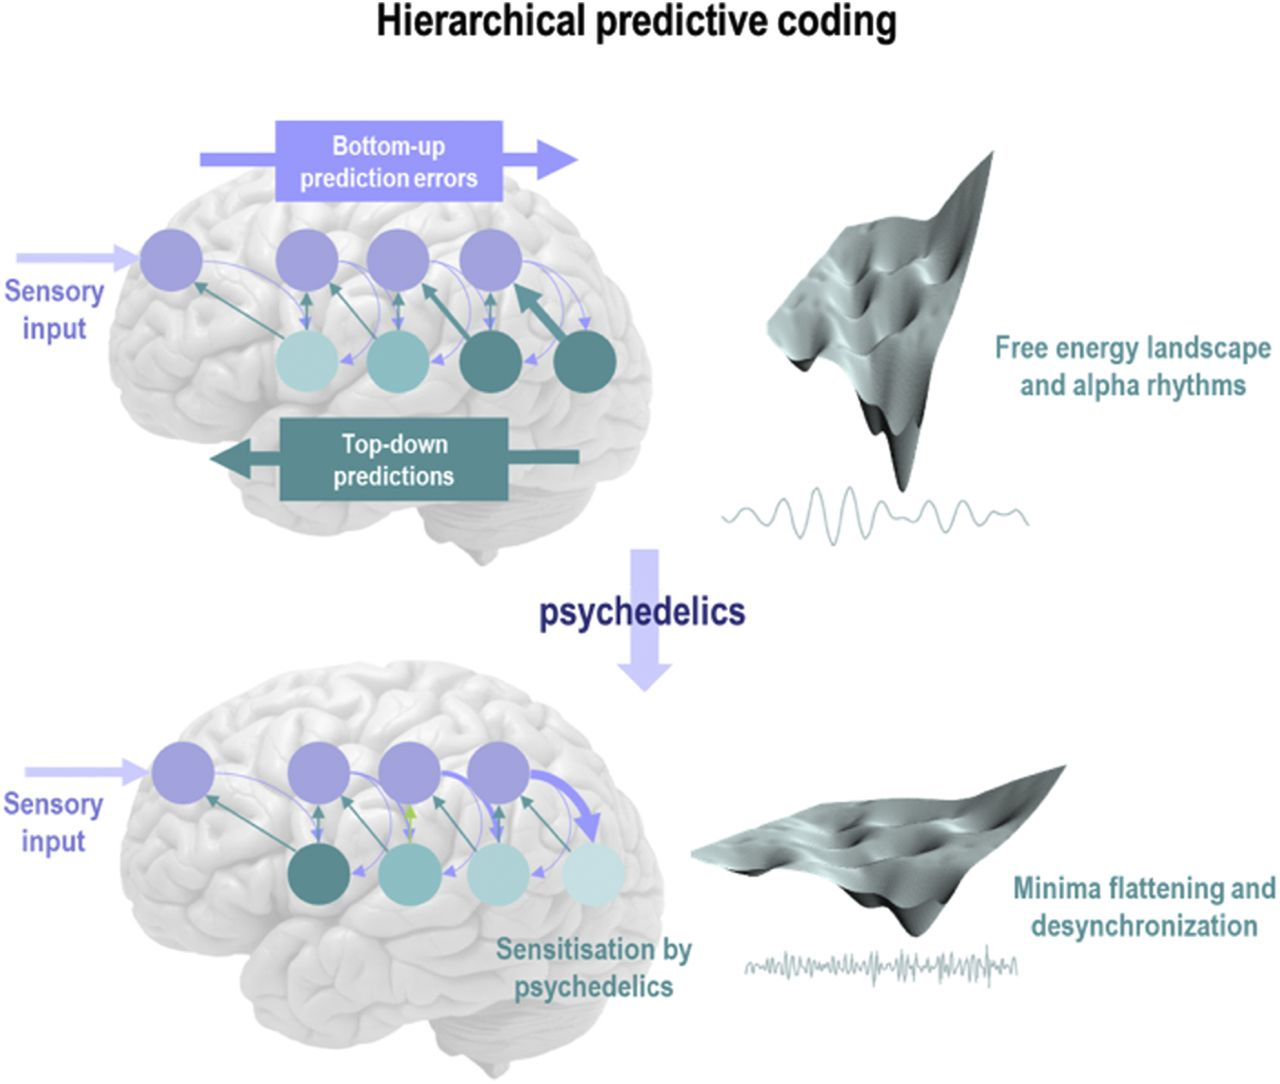
\includegraphics[height=4.cm]{img/F1.large.jpg}
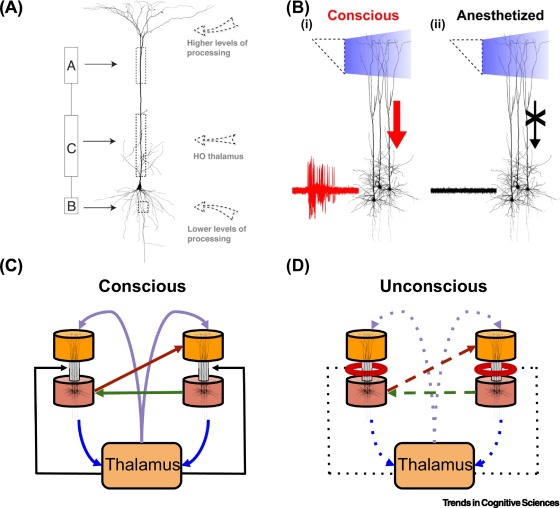
\includegraphics[height=4.cm]{img/gr2.jpeg}
\end{frame}



%%%%%%%%%%%%%%%%%%%%%%%%%%%%%%%%%%%%%%%%%%%%%%%%%%
\begin{frame}[label=ladila]{Model-building: life}
 How do agents build models? In addressing this, the algorithmic framework connects the concepts of life, intelligence, and \SEP. \vfill
 
 Both life and intelligence represent processes to construct simple models for the persistence of algorithmic information-preserving systems across time. \vfill
 
  Starting from resilient building blocks (static persistence), from a computational perspective {\em life} is an algorithmic process: program building carried not solely by the individual agent, but by the transgenerational agent through evolution (v. also \cite{Walker2013, Chaitin2012-wd}).
  
\end{frame}

%%%%%%%%%%%%%%%%%%%%%%%%%%%%%%%%%%%%%%%%%%%%%%%%%%
\begin{frame}[label=ladila]{Model-building: intelligence}
 Evolutive pressure gives rise to the next leap, {\em intelligence}: agents that, starting from their static model (DNA in life) can actually build higher-level compressive models of the world within their lifetime, e.g., using brains.\vfill
 
 Importantly, KT holds that both static-model and active-modeling agents enjoy structured experience, only that their level of structure is possibly different.  \vfill
 
 
 [What comes after life and intelligence?]
 
\end{frame}


%%%%%%%%%%%%%%%%%%%%%%%%%%%%%%%%%%%%%%%%%%%%%%%%%%
\begin{frame}[label=ladila]{Model-building in artificial agents}
As a consequence of the above, two routes to the construction of model-building agents   (virtual or physical)  should be investigated: \vfill

A) {\bf Single generation} model building where agents are endowed with simplicity biases for model building (this is what we call the  {\em intelligence} approach). \vfill


B) {\bf Trans-generational} model building ({\em life}) where the bias for simplicity is not added by hand but emerges naturally from the construction process that favors simple short programs (and which then lead to phenotype symmetry as in \citep{Johnston2022})  and evolutionary pressure in {\em  environments governed by simple laws}.  
\end{frame}